\section{Theoretical Analysis}
\label{sec:analysis}

Since the input voltage is Vs = 230V but the desired output is 12V, we used a tranformer to reduce the voltage to the desired value, given the expression Vr = Vs/n, with n = 10. However,
we still have to conver the Alternated Current into Direct Current. To do this, the circuit shown in Figure~\ref{fig:cir} was used.

This circuit is composed by three main subcircuits, already meantioned in the introduction. 

The four diodes numbered from 1 to 4 form the Full-Wave Rectifier. They have the function of converting the AC voltage into direct current, by allowing only for a unidirectional flow, as show in green in
 Figure~\ref{fig:output}. This is equal to the absolute value of Vr. 

The capacitor is utilized to reduce the magnitude of the voltage, making it closer DC voltage and reducing the "ripple", as shown in COLOR, in Figure~\ref{fig:output}.
This can be computed by determining when the diodes are ON an OFF. Periodically, we get:

\begin{equation}
    \begin{cases}
        vO = Vr \qquad , t < t_{OFF} \\
	    vO = Vs \cdot cos(w \cdot t_{OFF}) \cdot exp(-\frac{t-t_{OFF}}{R_{eq} \cdot C}) \qquad , t > t_{OFF}.
    
  \label{eq:vo}  
  \end{cases}
\end{equation}


Finally,the 20 diodes in series are used for the purpose of reducing the noise, making the plot even closer to DC, as shown in COLOR, in Figure~\ref{fig:output}.
 By calculating the Vo average, one can see if the voltage drop at the diodes terminals is limited by the maximum voltage that those diodes can handle. 
This is the case when that average is greater than that maximum. After this, we are left with a voltage due to the DC component, 
so we still need to take into account the AC component. This can be computed by calculating Rd (the resistance of each diode), which depends on the diode material properties.

Then, the AC component is given by:

$vO_{AC} = number of diodes \cdot \frac{rd}{number of diodes \cdot rd+R2} \cdot (vO_{envelope}-average_{envelope})$

With this, vO is simply given by: $vO$ = $vO_{DC}$ + $vO_{AC}$.

This value should be close to 12V.

\begin{table}[ht]
  \centering
  \begin{tabular}{|l|r|}
    \hline    
    {\bf Name} & {\bf Value} \\ \hline
	Ripple(envelope) & 4.100025e-01 \\ \hline
Average(envelope) & 2.279872e+01 \\ \hline

  \end{tabular}
  \caption{Ripple and average envelope values}
	\label{tab:envelope}
\end{table}

\begin{table}[ht]
  \centering
  \begin{tabular}{|l|r|}
    \hline    
    {\bf Name} & {\bf Value} \\ \hline
        regulatorripple & 6.729519e-02 \\ \hline
regulatoraverage & 1.200000e+01 \\ \hline

  \end{tabular}
  \caption{Ripple and average regulator values} 
        \label{tab:regulator}
\end{table}     



\begin{figure}[h] \centering
\includegraphics[width=0.6\linewidth]{output.eps}
	\caption{Transformed input voltage, vr}
	\label{fig:output}
\end{figure}


\begin{figure}[h] \centering
\includegraphics[width=0.6\linewidth]{output2.eps}
	\caption{Envelope Detector and Voltage Regulator output voltages}
	\label{fig:output2}
\end{figure}

\begin{figure}[h] \centering                                          
\includegraphics[width=0.6\linewidth]{ac_component.eps}          
	\caption{Envelope detector and voltage regulator output voltages deviations around 12V}                                   
        \label{fig:ac_dc}                                            
\end{figure}







